
%(BEGIN_QUESTION)
% Copyright 2011, Tony R. Kuphaldt, released under the Creative Commons Attribution License (v 1.0)
% This means you may do almost anything with this work of mine, so long as you give me proper credit

{\it Nernst-ligningen} brukes i mange ulike kjemiske analyseteknologier. En av disse er måling av {\it oksygenkonsentrasjon} i blandede gassstrømmer, for eksempel avgass fra en forbrenningsprosess der oksygeninnhold ofte holdes rundt 2\% (i stedet for atmosfærens normale 20.9\%). En vanlig oksygensensor består av et ``sandwich'' av platinaelektroder på hver side av en fast zirkoniumoksidmembran. Den ene siden av denne elektrokjemiske cellen eksponeres for avgassen (prosess), den andre for oppvarmet luft som referanse:

$$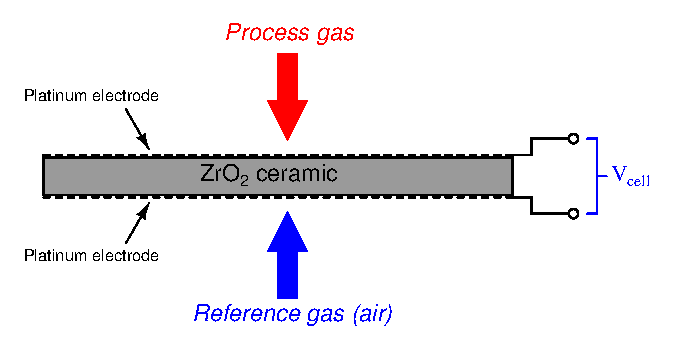
\includegraphics[width=15.5cm]{i00929x01.eps}$$

Spenningen fra cellen predikeres av Nernst-ligningen:

$$V = {{R T} \over {nF}} \ln \left({C_1 \over C_2}\right)$$

\noindent
Der,

$V$ = Spenning over membranen på grunn av ionebytte, i volt (V)

$R$ = Universell gasskonstant (8.315 J/mol$\cdot$K)

$T$ = Absolutt temperatur, i kelvin (K)

$n$ = Antall elektroner overført per utvekslet ion (2 for oksygenatomer)

$F$ = Faradays konstant, i coulomb per mol (96,485 C/mol e$^{-}$)

$C_1$ = Oksygenkonsentrasjon i omgivelsesluft (20.9\%)

$C_2$ = Oksygenkonsentrasjon i avgass

\vskip 10pt

Anta at en DAQ-modul er koblet til en slik oksygencelle, og du må legge inn en formel i DAQ-programvaren for å konvertere spenning til oksygenkonsentrasjon. Omform Nernst-ligningen og løs for oksygenkonsentrasjonen i avgassen ut fra målt spenning:

\vskip 30pt

$C_2$ = 

\vfil 

\underbar{file i00929}
\eject
%(END_QUESTION)





%(BEGIN_ANSWER)

Dette er en vurderingsoppgave -- ingen fasit eller hint oppgis!

%(END_ANSWER)





%(BEGIN_NOTES)

Nøkkelen til å løse ligningen for $C_2$ er å ``oppheve'' naturlig logaritme. Husk at hver aritmetisk funksjon har en invers: addisjon oppheves med subtraksjon, multiplikasjon med divisjon, og logaritme med eksponentialfunksjon. For naturlig logaritme betyr det potens av $e$. Slik ser det ut:

$$V = {{R T} \over {nF}} \ln \left({C_1 \over C_2}\right)$$

$${VnF \over RT} =  \ln \left({C_1 \over C_2}\right)$$

$$e^{VnF \over RT} =  e^{\ln \left({C_1 \over C_2}\right)}$$

$$e^{VnF \over RT} =  {C_1 \over C_2}$$

$$C_2 = {C_1 \over e^{VnF \over RT}}$$

Hvis vi vet at hvert oksygenion har dobbelt negativ ladning, kan vi sette $n = 2$ for denne applikasjonen:

$$C_2 = {C_1 \over e^{2VF \over RT}}$$

%INDEX% Mathematics review: manipulating literal equations

%(END_NOTES)

